\section{Introduction}

\begin{frame}[fragile]{} 
\begin{center}
\begin{figure}
  \centering
  \subfloat{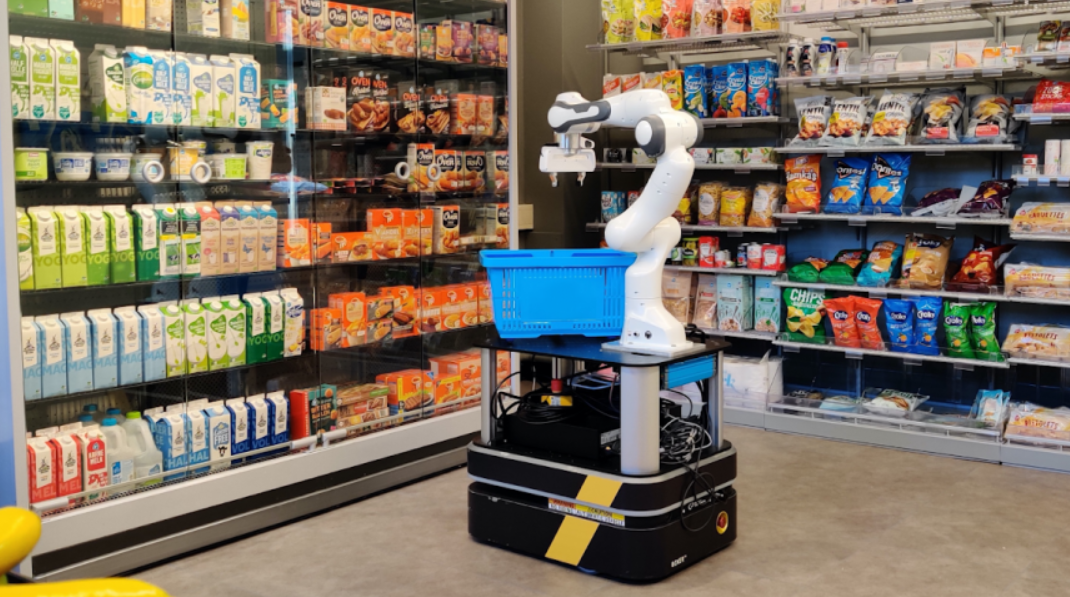
\includegraphics[width=0.44\textwidth]{figures/introduction/robot2}}\quad
  \subfloat{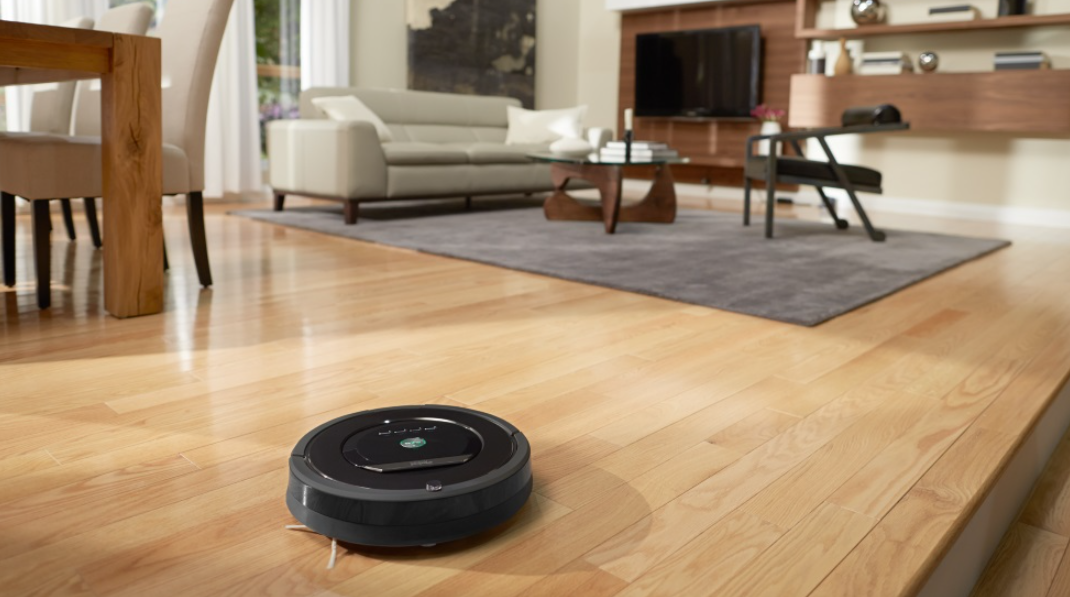
\includegraphics[width=0.44\textwidth]{figures/introduction/robot4}}

  \subfloat{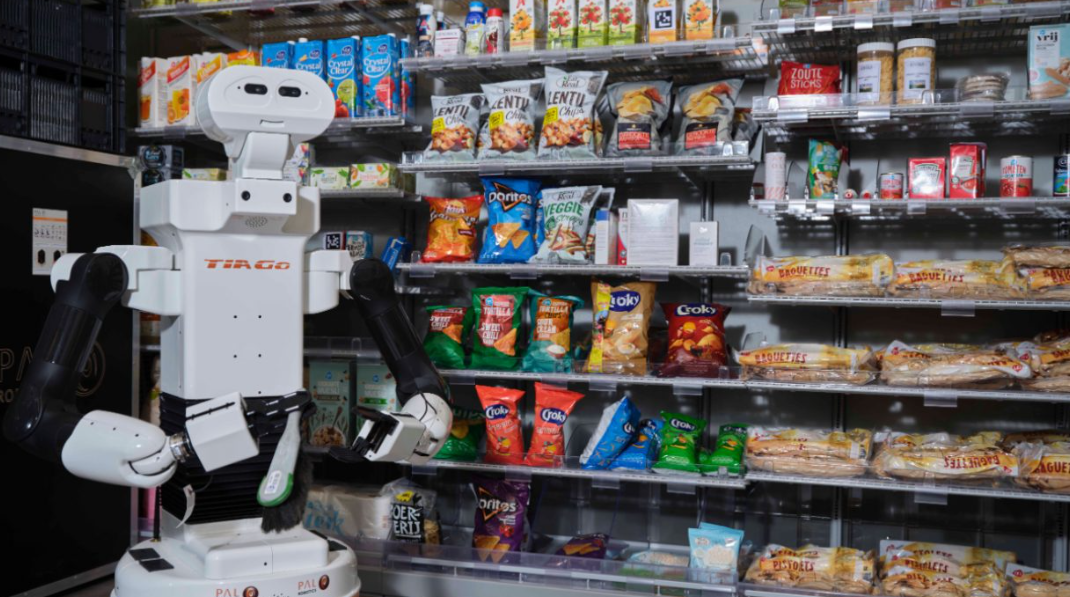
\includegraphics[width=0.45\textwidth]{figures/introduction/robot3}}
\end{figure}
\end{center}
\end{frame}

\begin{frame}[c]{Intro} 
  \begin{block}{Challenges}
    \begin{enumerate}
      \item Controllers 
      \item Different Environments
      \item Many System Models of objects
    \end{enumerate}
  \end{block}
\end{frame}

\begin{frame}[c]{Intro} 
  \begin{block}{Table of Content}
    \begin{enumerate}
      \item Introduction
      \item Required Background
      \item Proposed Method
      \item Results
      \item Conclusions
    \end{enumerate}
  \end{block}
\end{frame}

\begin{frame}[fragile]{Intro} 
\begin{block}{}
\begin{itemize}
  \item Learn System Models\\
  \item Select best Available Controller
\end{itemize}
  \end{block}\pause

\begin{block}{}
\begin{itemize}
  \item Navigation Among Movable Objects (NAMO)\\
  \item Nonprehensile Pushing
\end{itemize}
  \end{block}
\end{frame}

\vspace{0.3cm}
\centering
\begin{tikzpicture}[scale=1.05, every node/.style={scale=1.05}, node distance = 2cm, auto]
   
  \node [outer sep=0cm] (environment) at (0,0)  {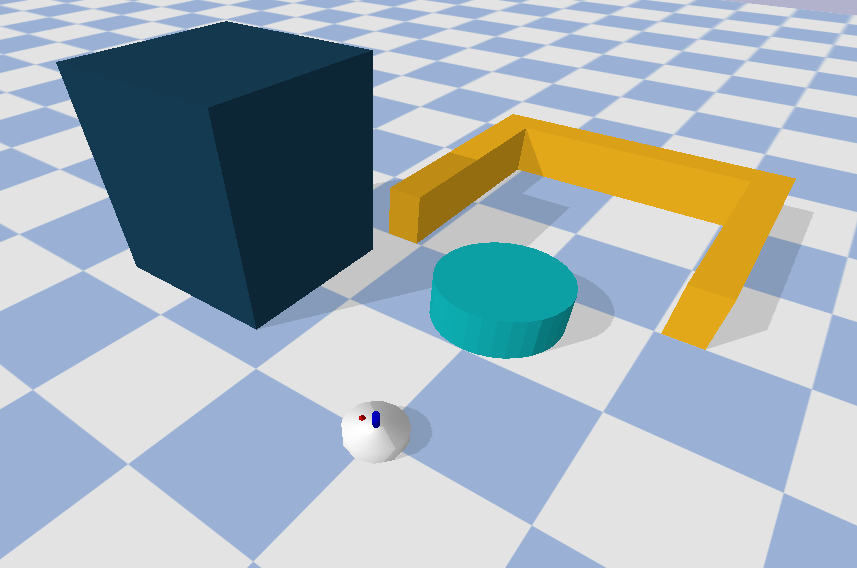
\includegraphics[width=4.6cm]{figures/introduction/blockade}}; overvew

  \draw [myEvenLighterColor,
  rounded corners=0.3cm, 
  line width=0.3cm]  
  (environment.north west) -- 
  (environment.north east) --
  (environment.south east) --
  (environment.south west) -- cycle  ;

  \node [block,
  above of=environment,
  minimum height=2cm,
  minimum width=5cm,
  node distance=4.1cm,
  outer sep=0cm] (hgraph) {Proposed Robot Framework};

  % Draw edges
  \draw[-stealth] ([yshift=0.155cm, xshift=0.4 cm]environment.north) -- node [xshift=-.05cm, right] {\shortstack[]{sensor\\measurements}}([xshift=0.4 cm]hgraph.south) ;
  \draw[-stealth] ([xshift=-0.4 cm]hgraph.south) -- node [left] {robot input}([yshift=0.155cm, xshift=-0.4 cm]environment.north) ;
  \draw[stealth-] (hgraph.west) -- node [above] {task} ++(-1, 0);

\end{tikzpicture}




\begin{frame}[fragile]{Intro}
\vspace{-0.7cm}
\begin{center}
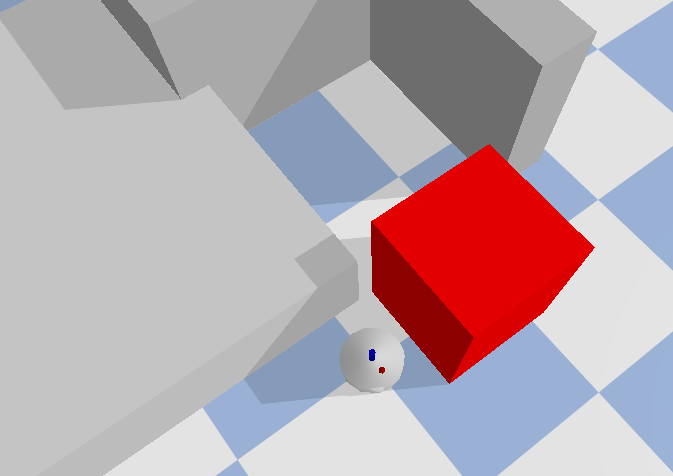
\includegraphics[height=0.9\textheight]{figures/introduction/robot_no_target}
\end{center}
\end{frame}

\begin{frame}[fragile]{Intro}
\vspace{-0.7cm}
\begin{center}
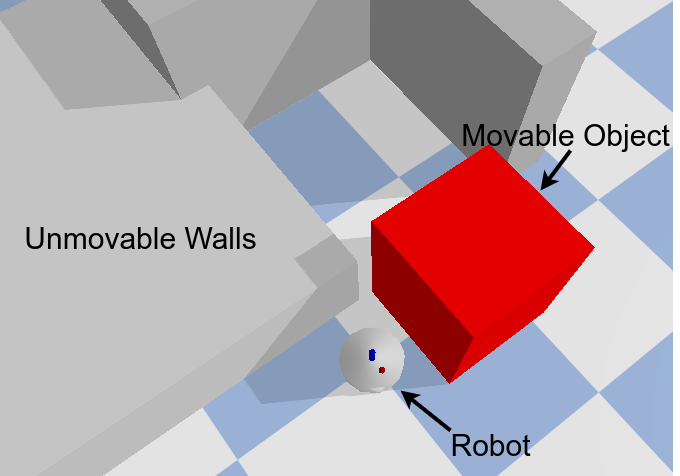
\includegraphics[height=0.9\textheight]{figures/introduction/robot_no_target_with_arrows}
\end{center}
\end{frame}

\begin{frame}[fragile]{Intro}
\vspace{-0.7cm}
\begin{center}
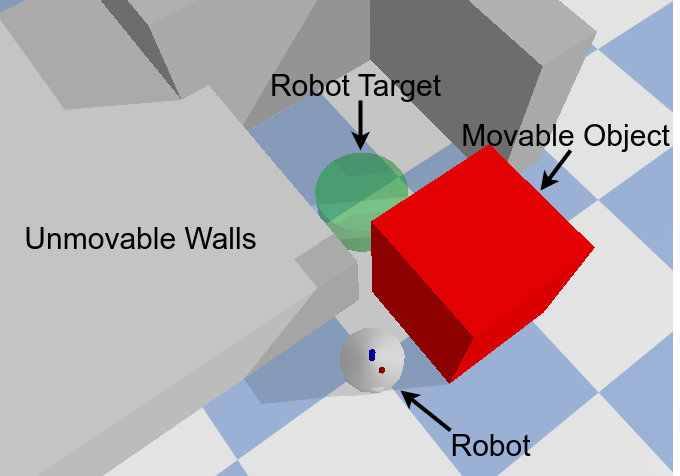
\includegraphics[height=0.9\textheight]{figures/introduction/robot_with_target}
\end{center}
\end{frame}

% \begin{frame}[fragile]{Intro}
%   \begin{minipage}[l]{0.46\textwidth}
%     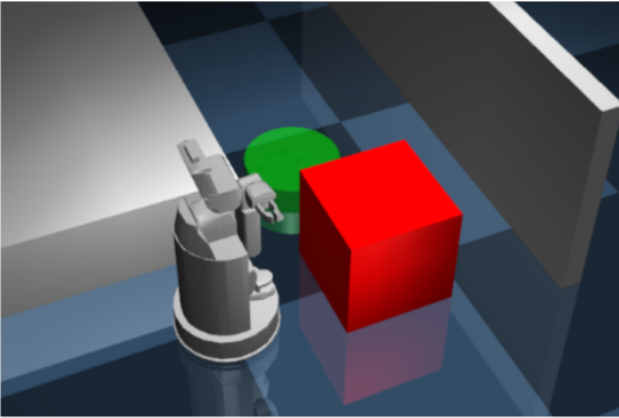
\includegraphics[width=1.3\textwidth]{figures/introduction/wang}
%   \end{minipage}\pause
%   \begin{minipage}[l]{0.3\textwidth}
%     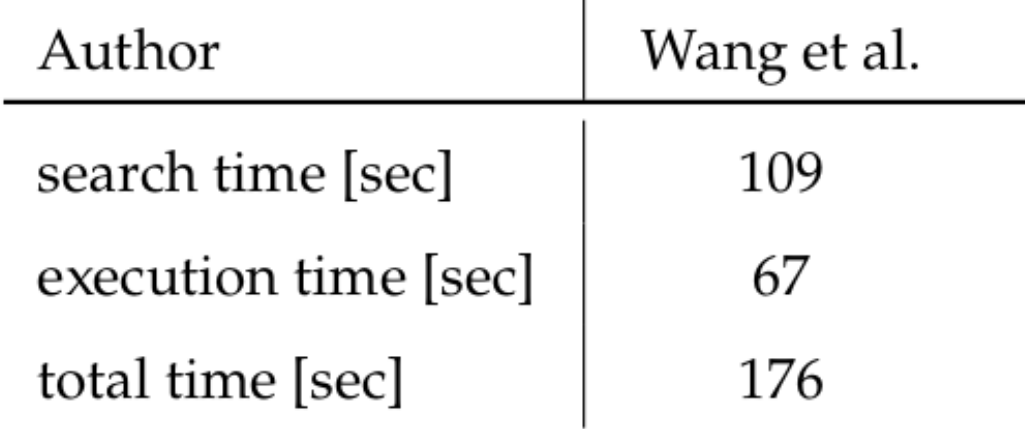
\includegraphics[width=1.8\textwidth]{figures/introduction/wang_table}
%     \vspace{3.0cm}
%   \end{minipage}
%   \cite{wang_affordancebased_2020}
% \end{frame}

\begin{frame}[fragile]{Intro}
  \begin{minipage}[l]{0.46\textwidth}
    \cite{wang_affordancebased_2020}
    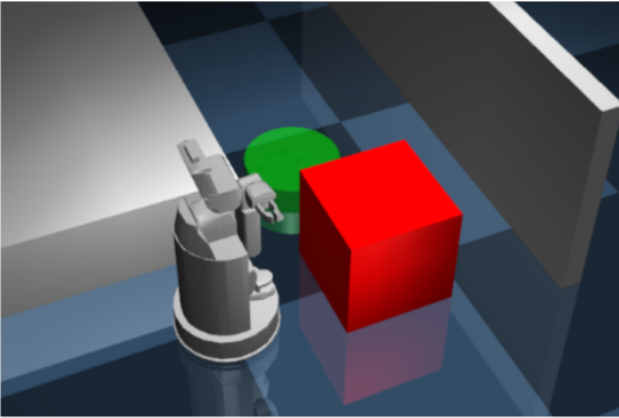
\includegraphics[width=1.3\textwidth]{figures/introduction/wang}
  \end{minipage}
  \begin{minipage}[l]{0.3\textwidth}
\begin{overprint}
  \onslide<1> 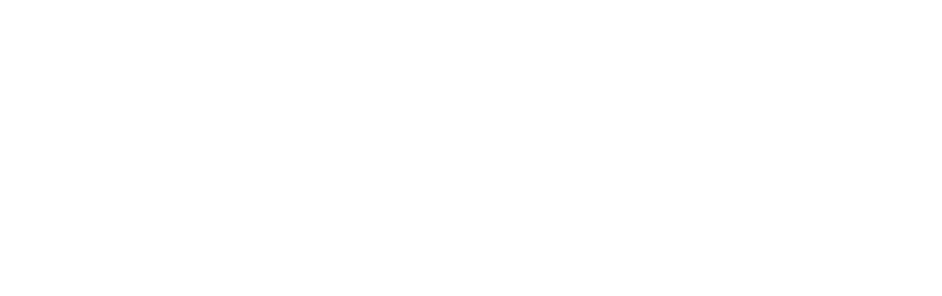
\includegraphics[width=1.8\textwidth]{figures/introduction/wang_table_transparent}\vspace{3.5cm}
  \onslide<2> 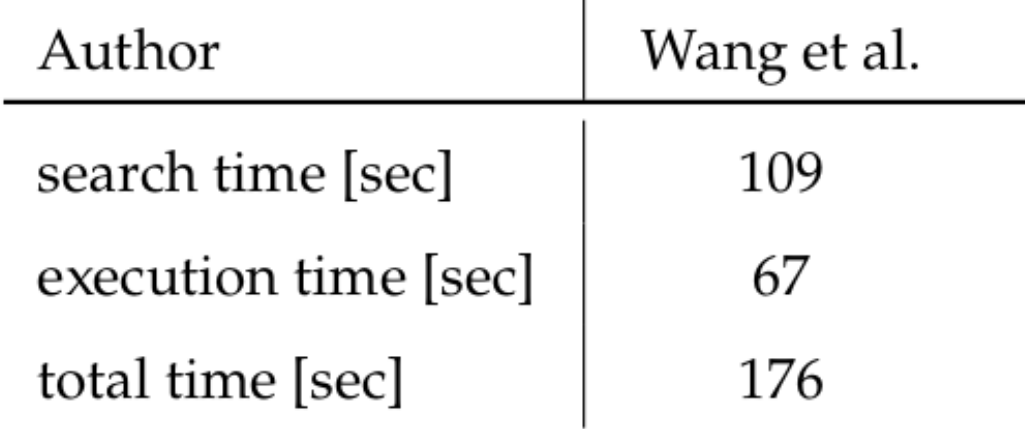
\includegraphics[width=1.8\textwidth]{figures/introduction/wang_table}\vspace{3.5cm}
    \onslide<3> 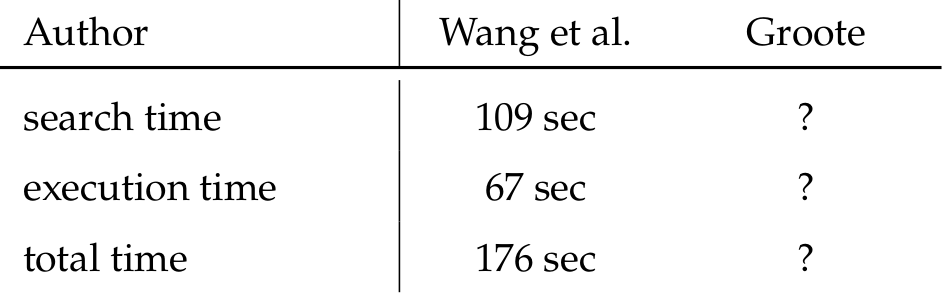
\includegraphics[width=1.8\textwidth]{figures/introduction/wang_groote_table}\vspace{3.5cm}
\end{overprint}
  \end{minipage}
\end{frame}




\begin{frame}[fragile]{Intro}

  Research Question:\bs
  \begin{center}
  \large
  How to learn system models and how to select the\\ best available control method during task execution?\bs
  \end{center}
\end{frame}

\begin{frame}[fragile]{Intro}
  \begin{block}{Assumtions}
    \begin{enumerate}
      \item \textbf{Closed-World}\pause
      \item\textbf{Perfect Object Sensor}\pause
      \item\textbf{Tasks are Commutative}
    \end{enumerate}
  \end{block}
\end{frame}
